\documentclass[11pt]{beamer}
\usepackage{subcaption}
\usepackage{animate}
%Information to be included in the title page:
\title{Kimera: an Open-Source Library for Real-Time
Metric-Semantic Localization and Mapping} 
\author{Ken Schlesiger}
\institute{Universität Würzburg}
\date{25.01.2024}
\definecolor{arsenic}{rgb}{0.0666, 0.0666, 0.10588}
\definecolor{text}{rgb}{0.8039, 0.8392, 0.95686}
\definecolor{headlines}{HTML}{89b4fa}
\definecolor{flamingo}{HTML}{f0c6c6}
\definecolor{pink}{HTML}{f5bde6}
\pagecolor{arsenic}
\setbeamercolor{background canvas}{bg=arsenic}
\setbeamercolor{normal text}{fg=text}
\setbeamercolor{frametitle}{fg=headlines}
\setbeamercolor{titlecolor}{fg=headlines}
\setbeamercolor{title}{fg=pink}
\setbeamercolor{caption name}{fg=pink}
\color{text}
% Define the information for the footline

% Customize the footline
\begin{document}
\addtobeamertemplate{title page}{}{
  \begin{beamercolorbox}[sep=1em,wd=\paperwidth,leftskip=0.5cm,rightskip=0.5cm]{footlinecolor}
  \end{beamercolorbox}
}

\frame[plain]{\titlepage}

\begin{frame}
    \frametitle{Pose estimation and mesh reconstruction} 
    \begin{figure}[ht]
        \centering
        \animategraphics[width=\linewidth,autoplay,loop]{12}{kimera_VIO_gif/kimeravio_ROS_mesh-}{0}{256}
    \end{figure}
\end{frame}
\begin{frame}
\frametitle{Metric semantic mesh construction}
    \begin{figure}[ht]
        \centering
        \animategraphics[width=\textwidth,autoplay,loop]{20}{kimera_semantics_gif/kimera_semantics-}{0}{387}
    \end{figure}
\end{frame}
\begin{frame}
\frametitle{What does Kimera \cite{rosinol2020kimera} do?}
Three main Functions: 
\begin{itemize}
    \item Pose estimation (VIO) 
    \item 3D mesh reconstruction
    \item semantic mesh annotation
\end{itemize}
\end{frame}
\begin{frame}
\frametitle{The structure of Kimera}
\begin{figure}
    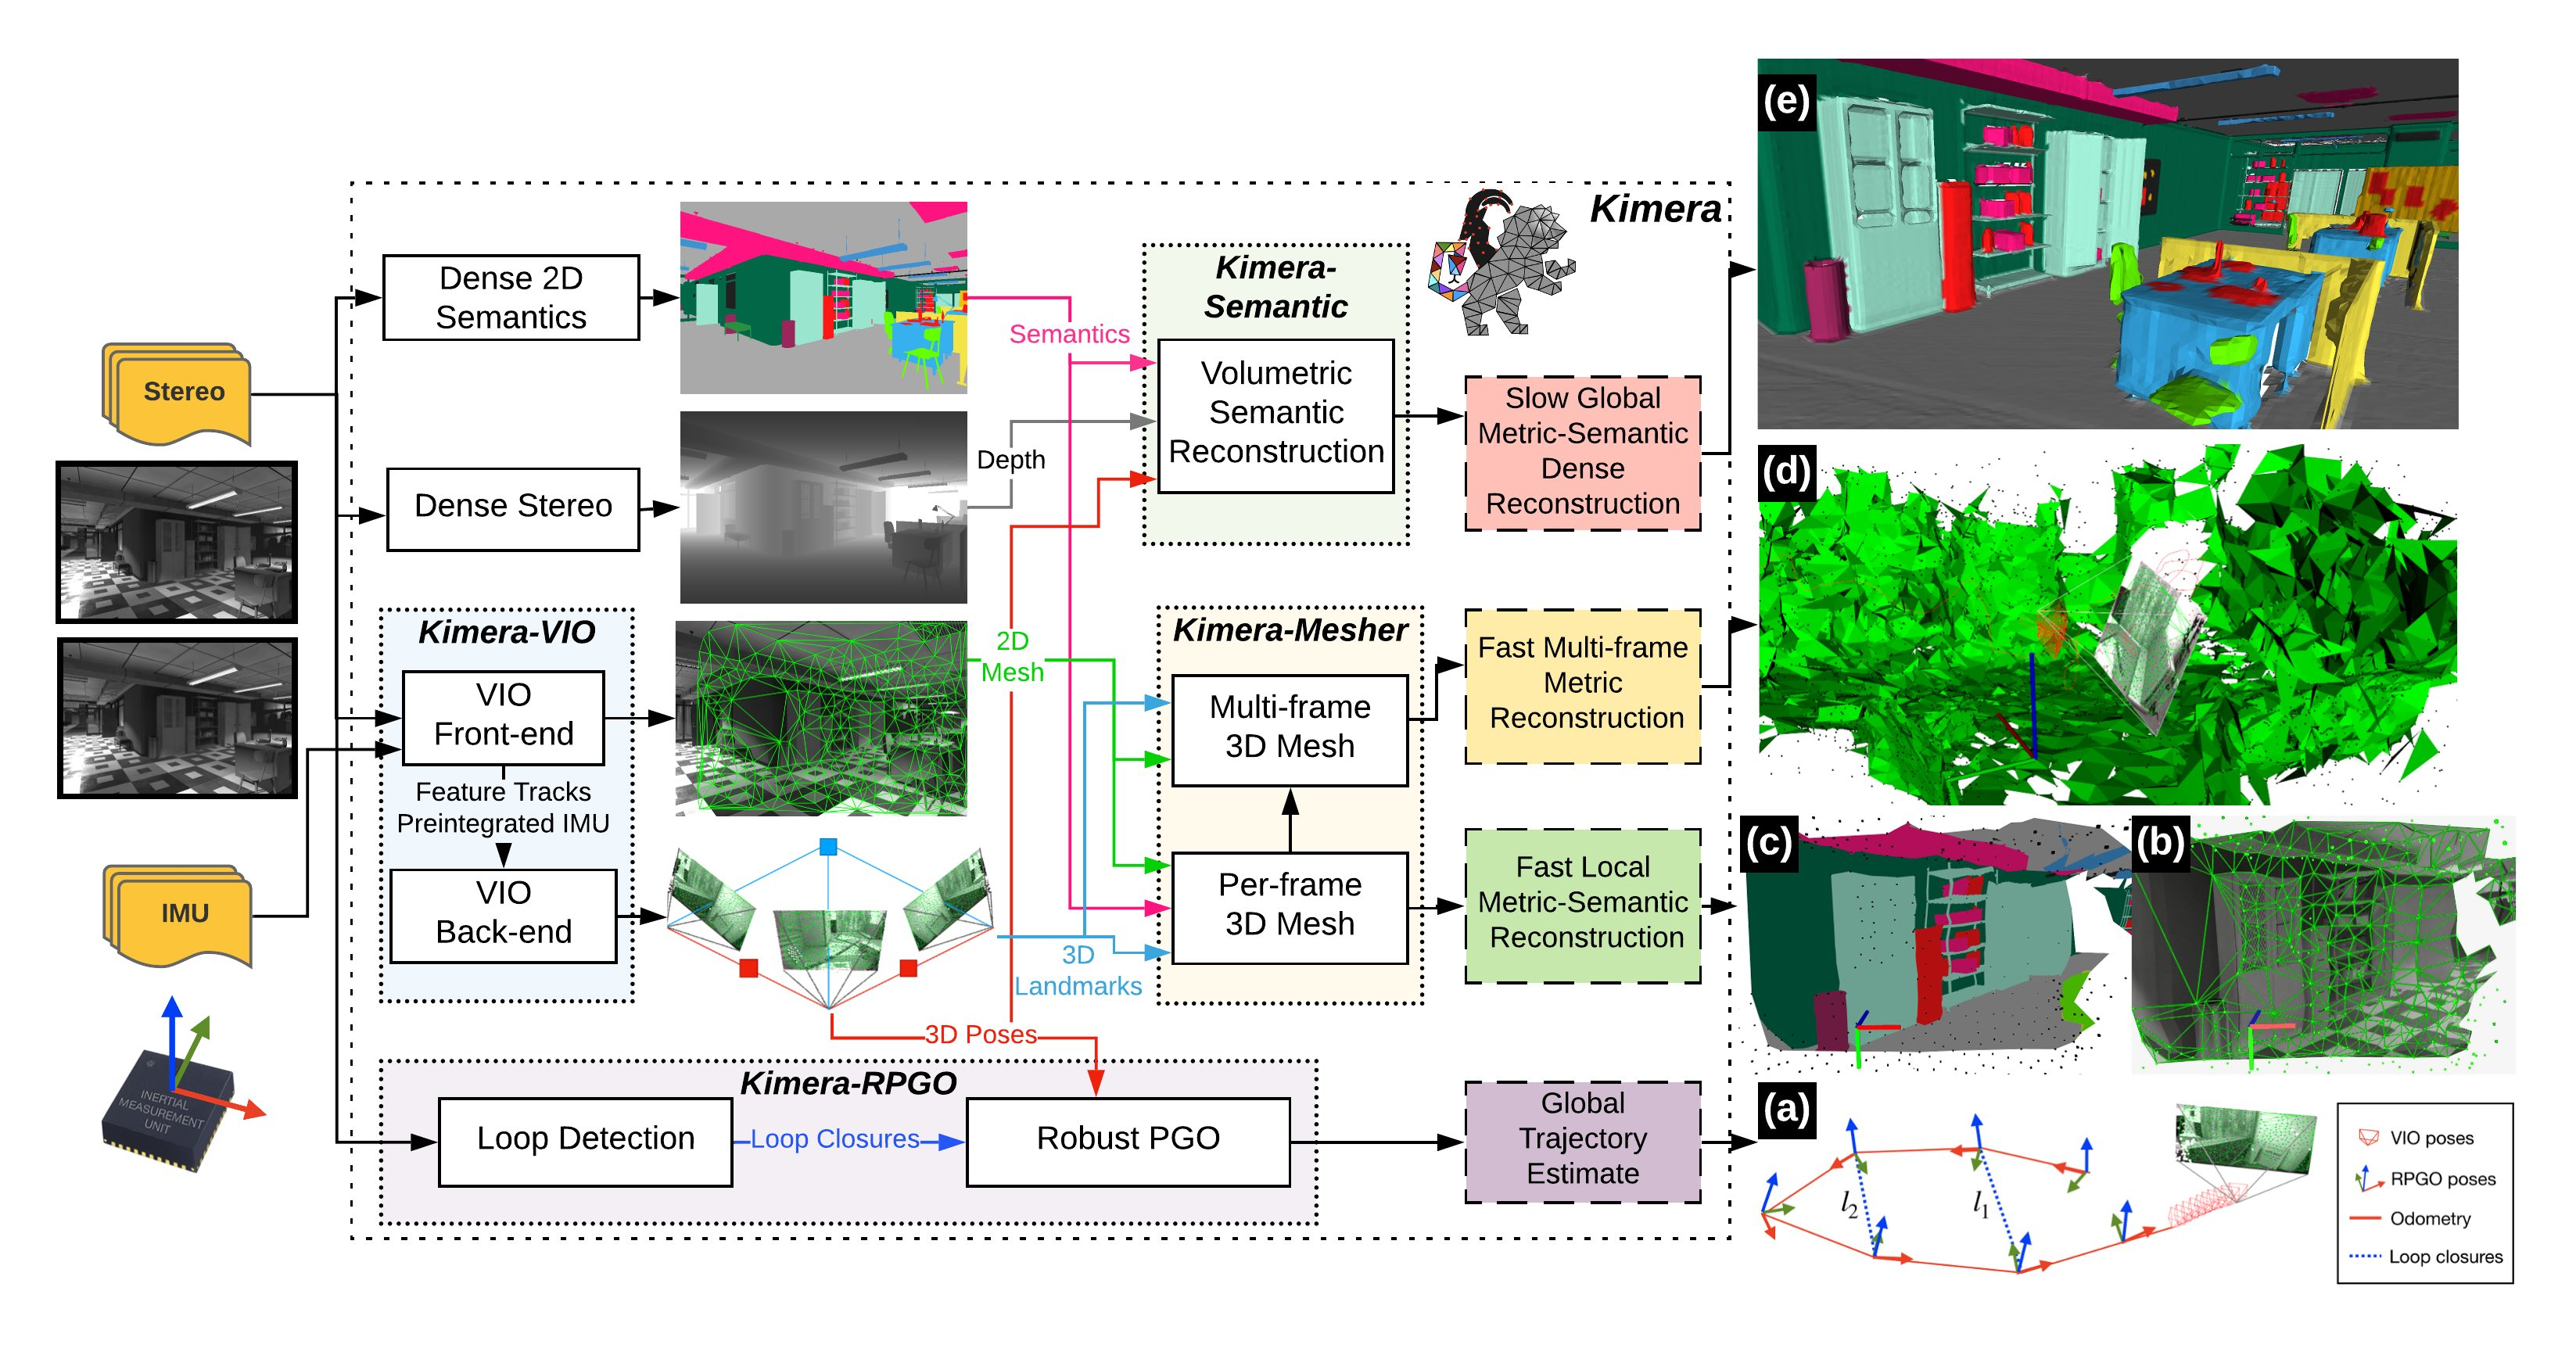
\includegraphics[width=\linewidth]{kimera_chart_23.jpeg} 
\end{figure}
\end{frame}
\begin{frame}
\frametitle{Kimera-VIO}
\begin{figure}
    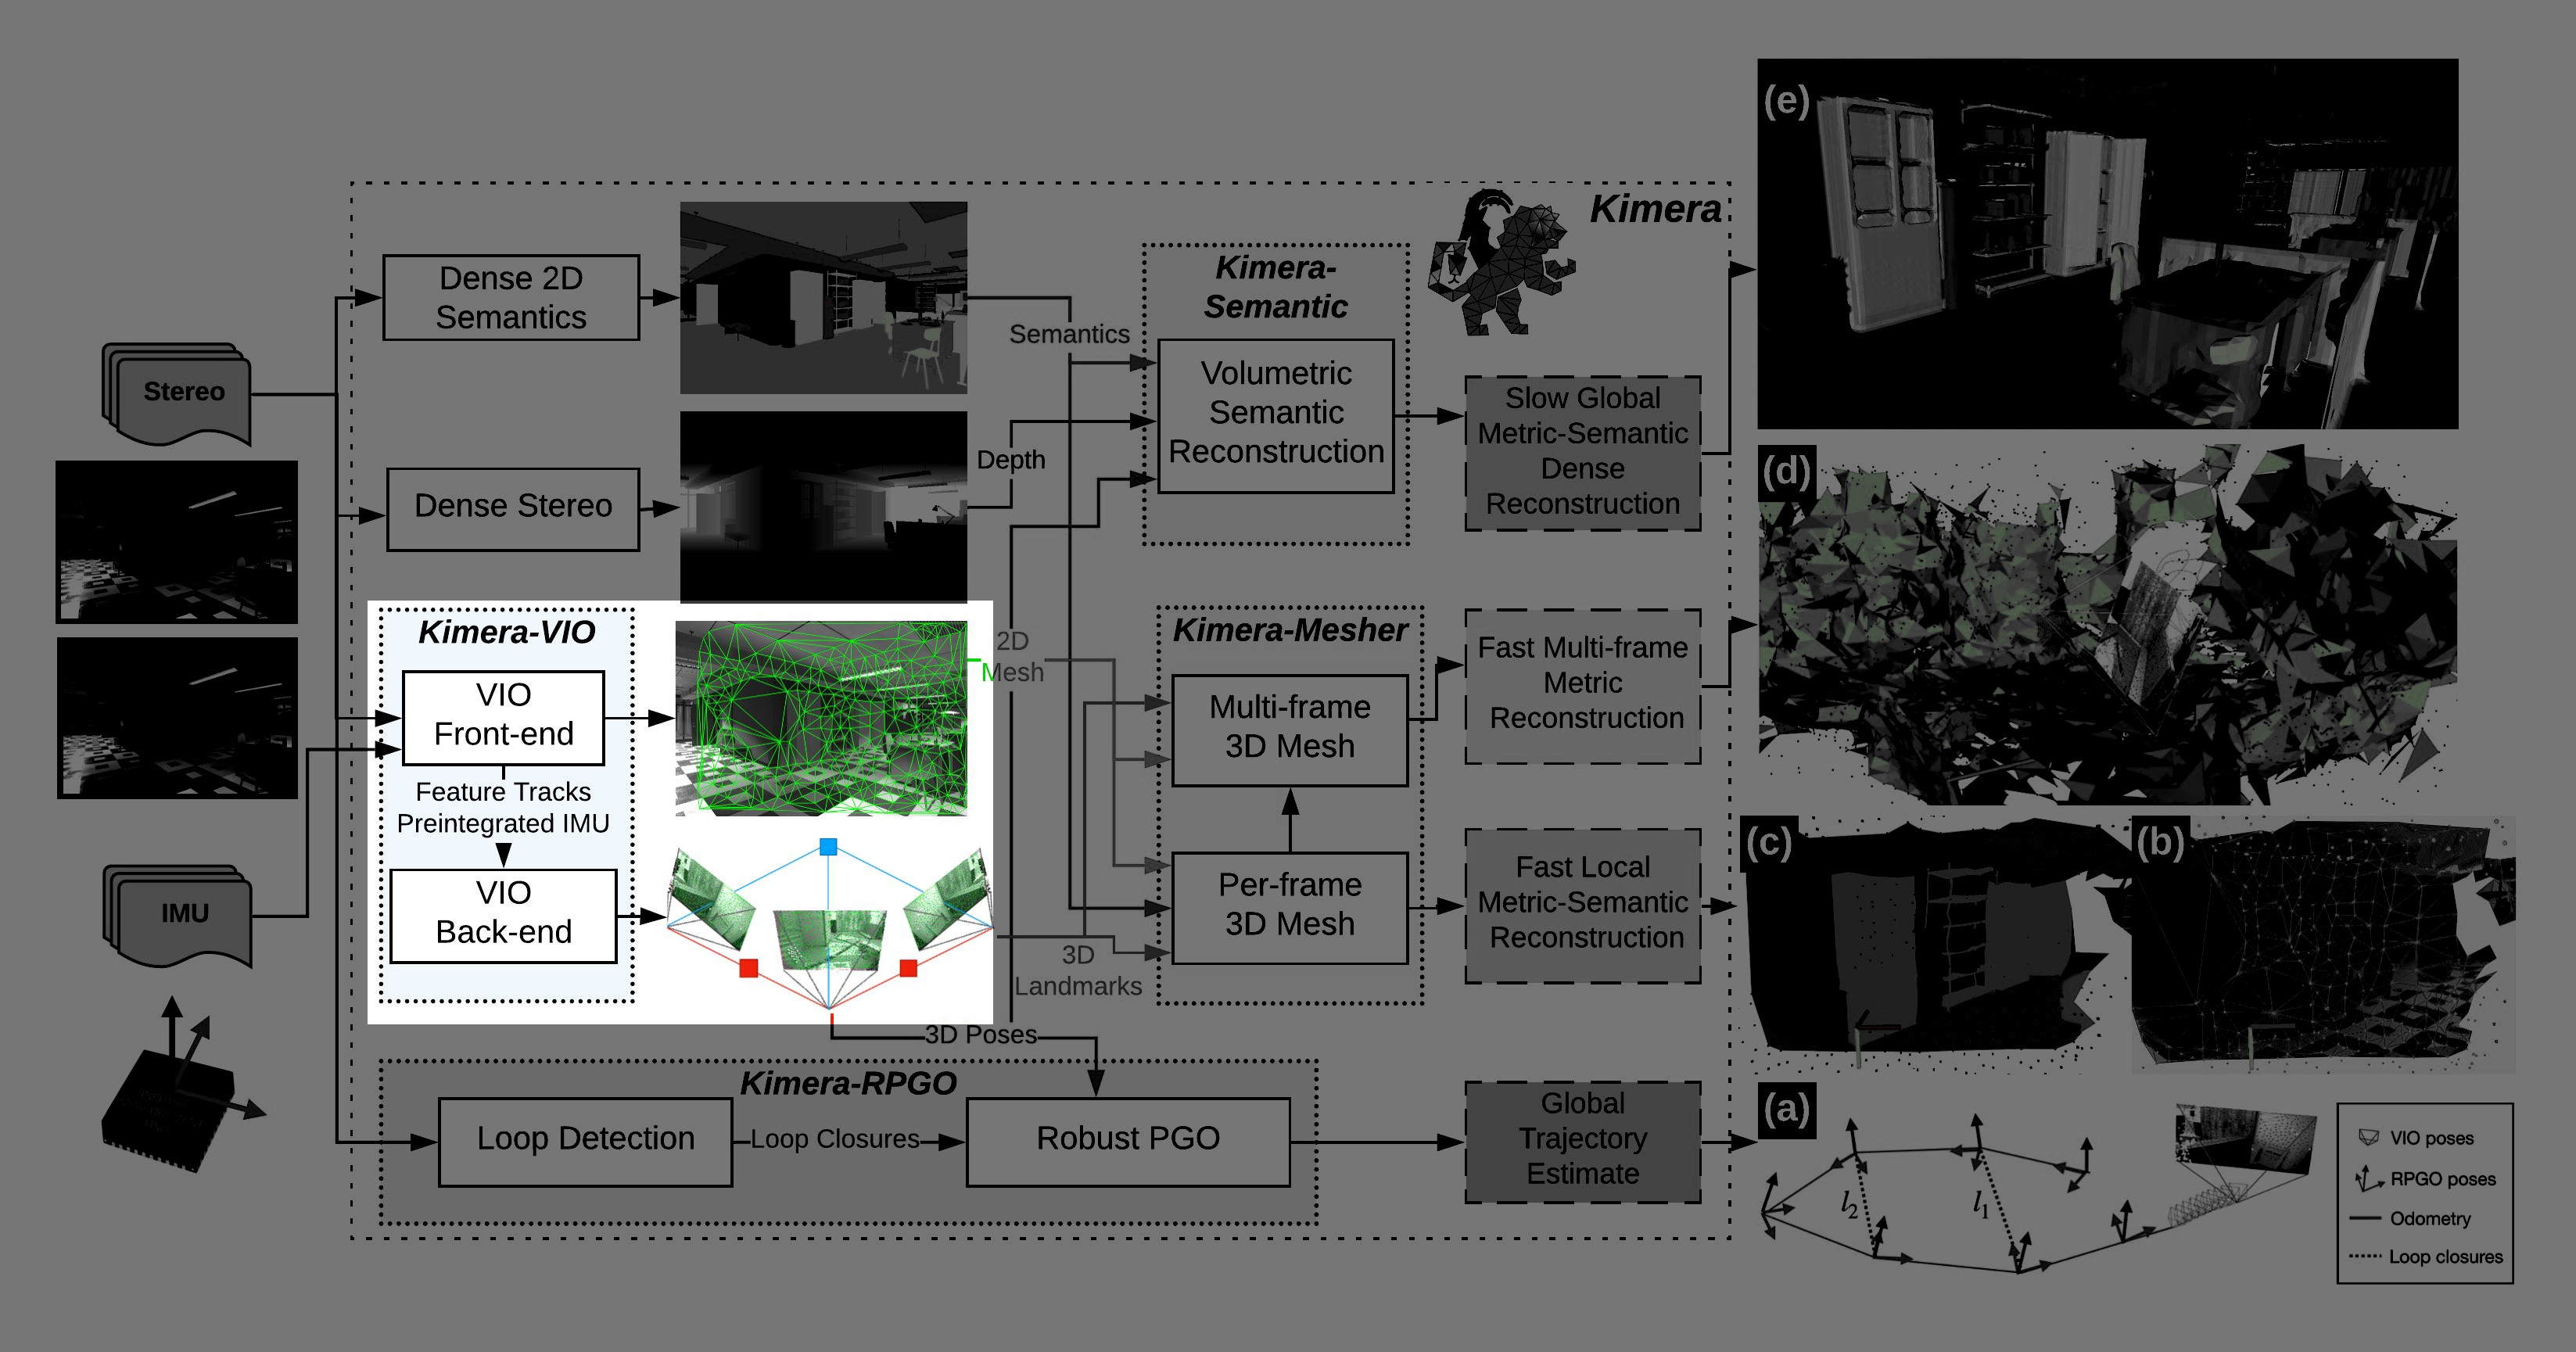
\includegraphics[width=\linewidth]{kimera_chart_VIO.jpeg} 
\end{figure}
\end{frame}
\begin{frame}
    \frametitle{Kimera-VIO} 
    \begin{figure}[ht]
        \centering
        \animategraphics[width=0.6\linewidth,autoplay,loop]{0.25}{kimera_VIO_gif/kimeravio_ROS_mesh-}{0}{47}
        \caption{Example of Corner Detection \cite{Shi_tomasi}}
    \end{figure}
Lucas Kanade \cite{lucas1981iterative} tracking:
\begin{align*}
           \begin{bmatrix}
               I_x (q_1) & I_y (q_1) \\ I_x (q_2) & I_y (q_2) \\  ... & ... \\I_x (q_n) & I_y (q_n)
           \end{bmatrix} 
           \begin{bmatrix}
               u \\ v
           \end{bmatrix} 
           = - 
           \begin{bmatrix}
               I_t (q_1) \\I_t (q_2) \\  ...\\I_t (q_n) 
           \end{bmatrix} 
\end{align*}
\end{frame}
\begin{frame}
\frametitle{The structure of Kimera}
\begin{figure}
    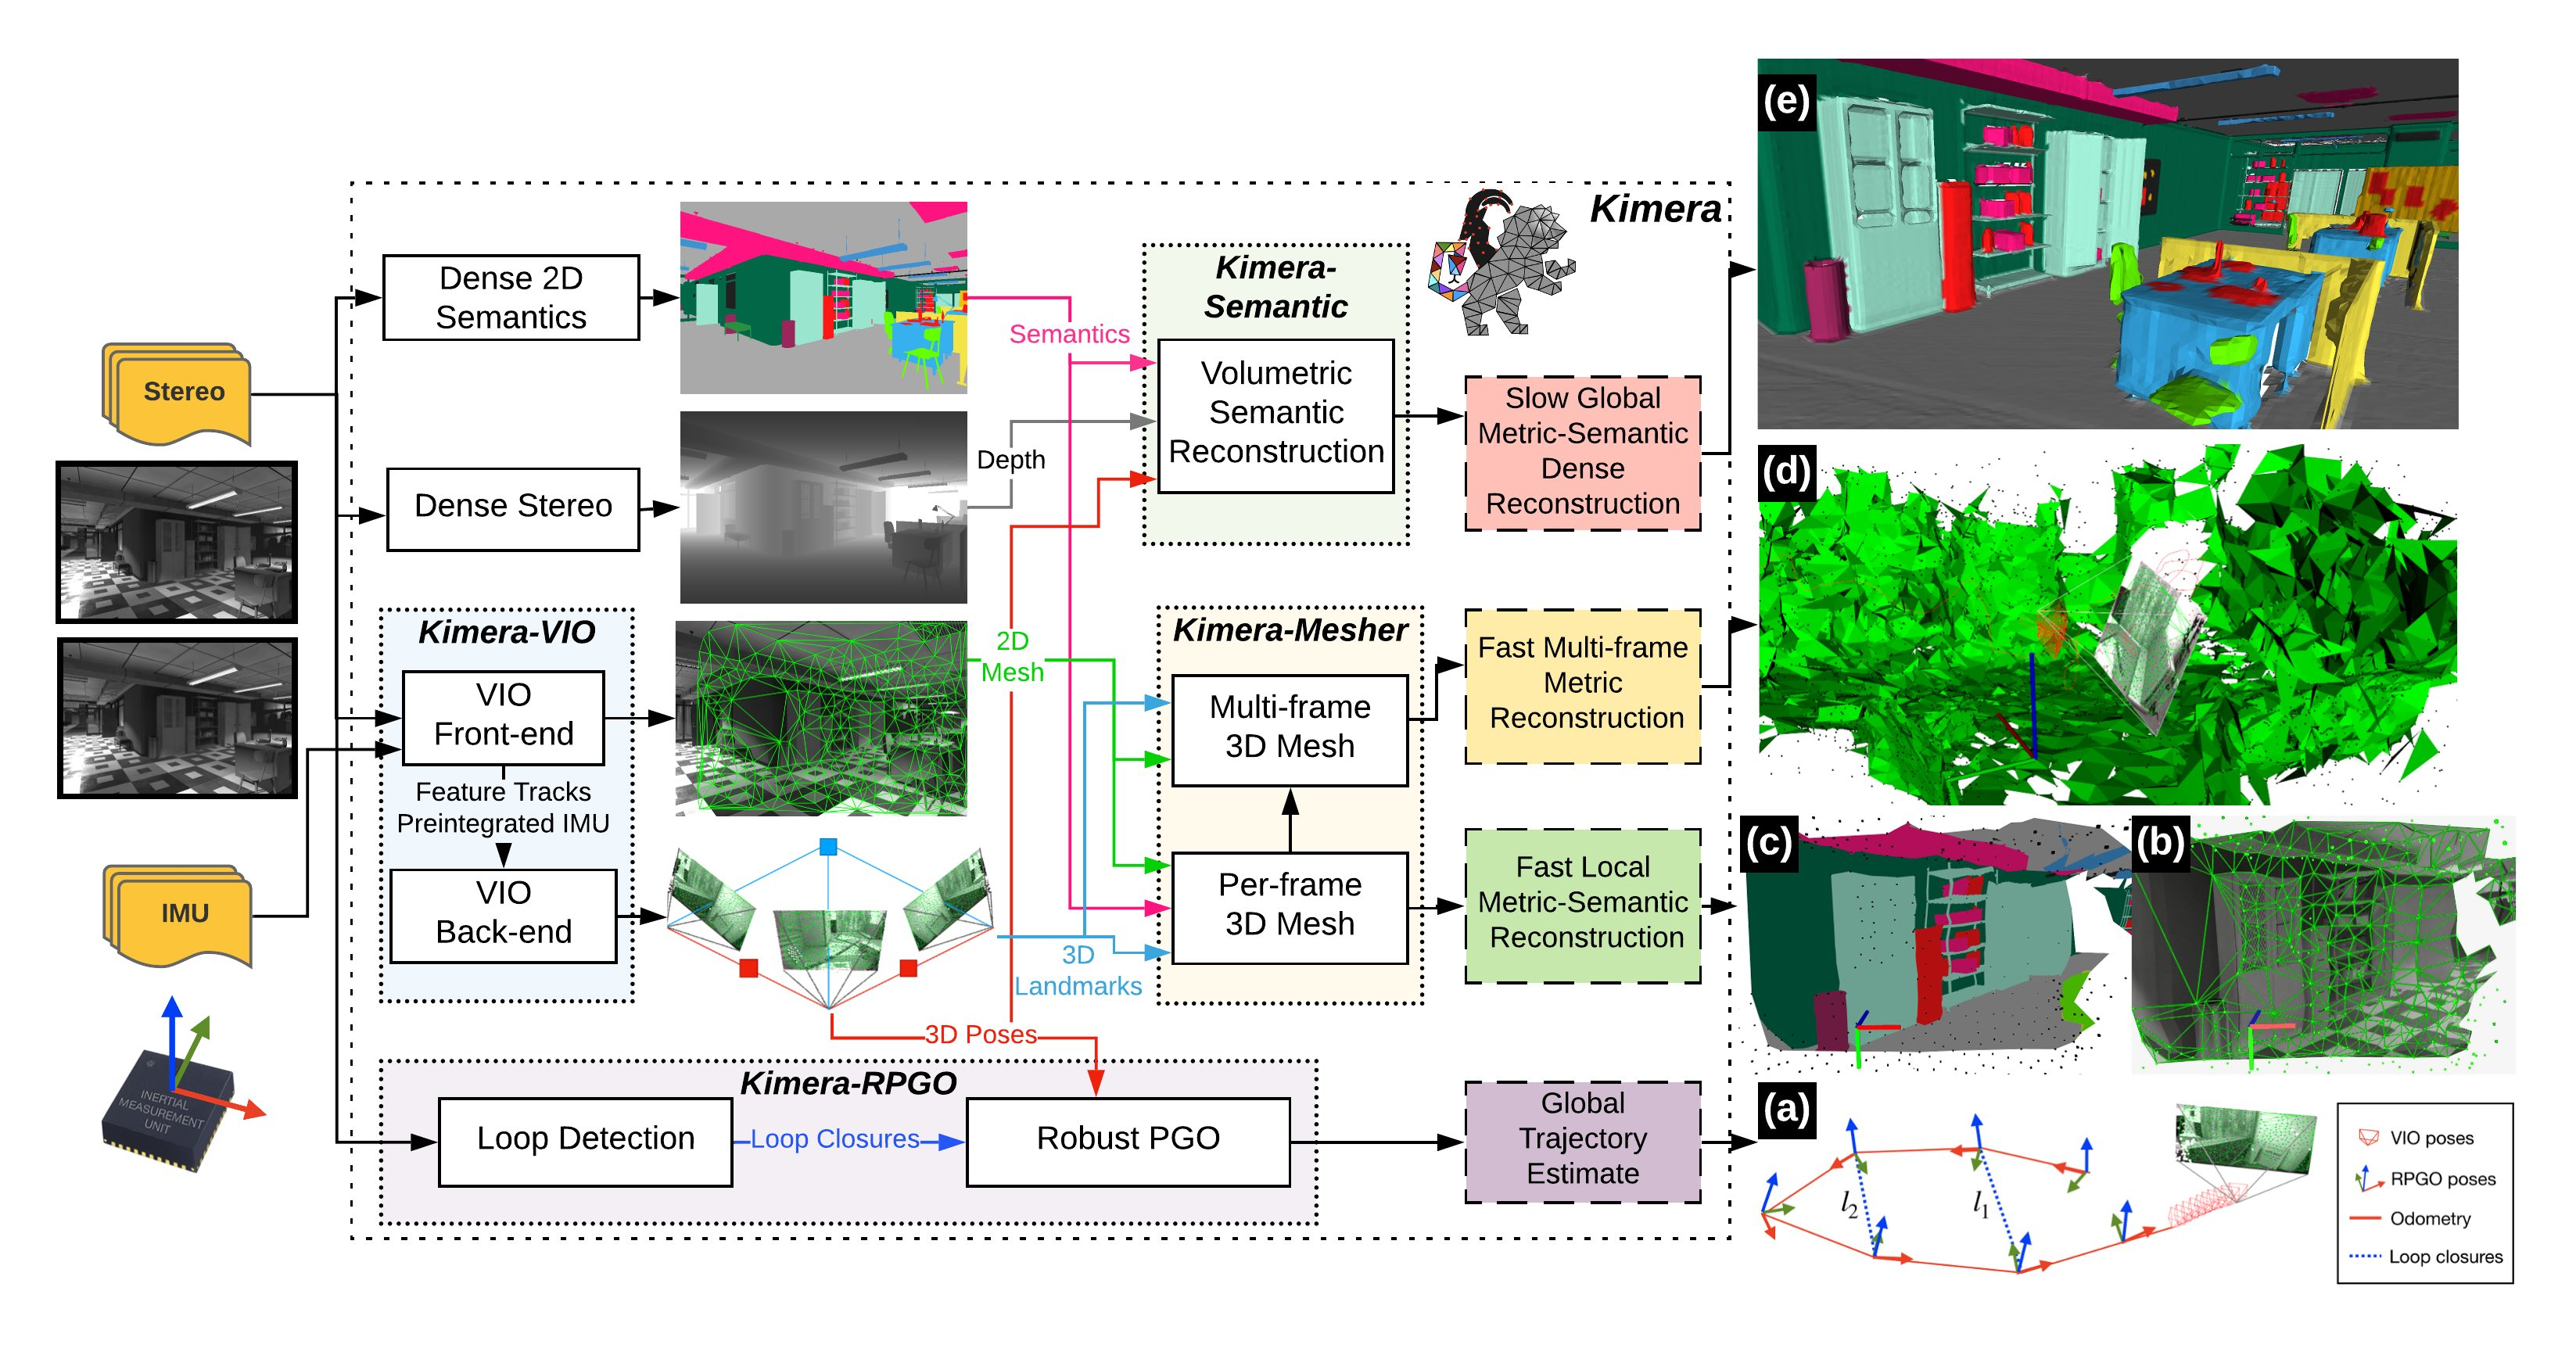
\includegraphics[width=\linewidth]{kimera_chart_23.jpeg} 
\end{figure}
\end{frame}
\begin{frame}
    \frametitle{Kimera-RPGO} 
\begin{figure}
    \includegraphics[width=\linewidth]{kimera_chart_RPGO.jpeg} 
\end{figure}
\end{frame}
\begin{frame}
    \frametitle{Kimera-RPGO} 
\begin{figure}
    \includegraphics[width=0.8\linewidth]{screenshot_2024-01-20-182926.png} 
    \caption{Incremental
    Consistent Measurement Set Maximization \cite{PCM}}
\end{figure}
\end{frame}
\begin{frame}
\frametitle{The structure of Kimera}
\begin{figure}
    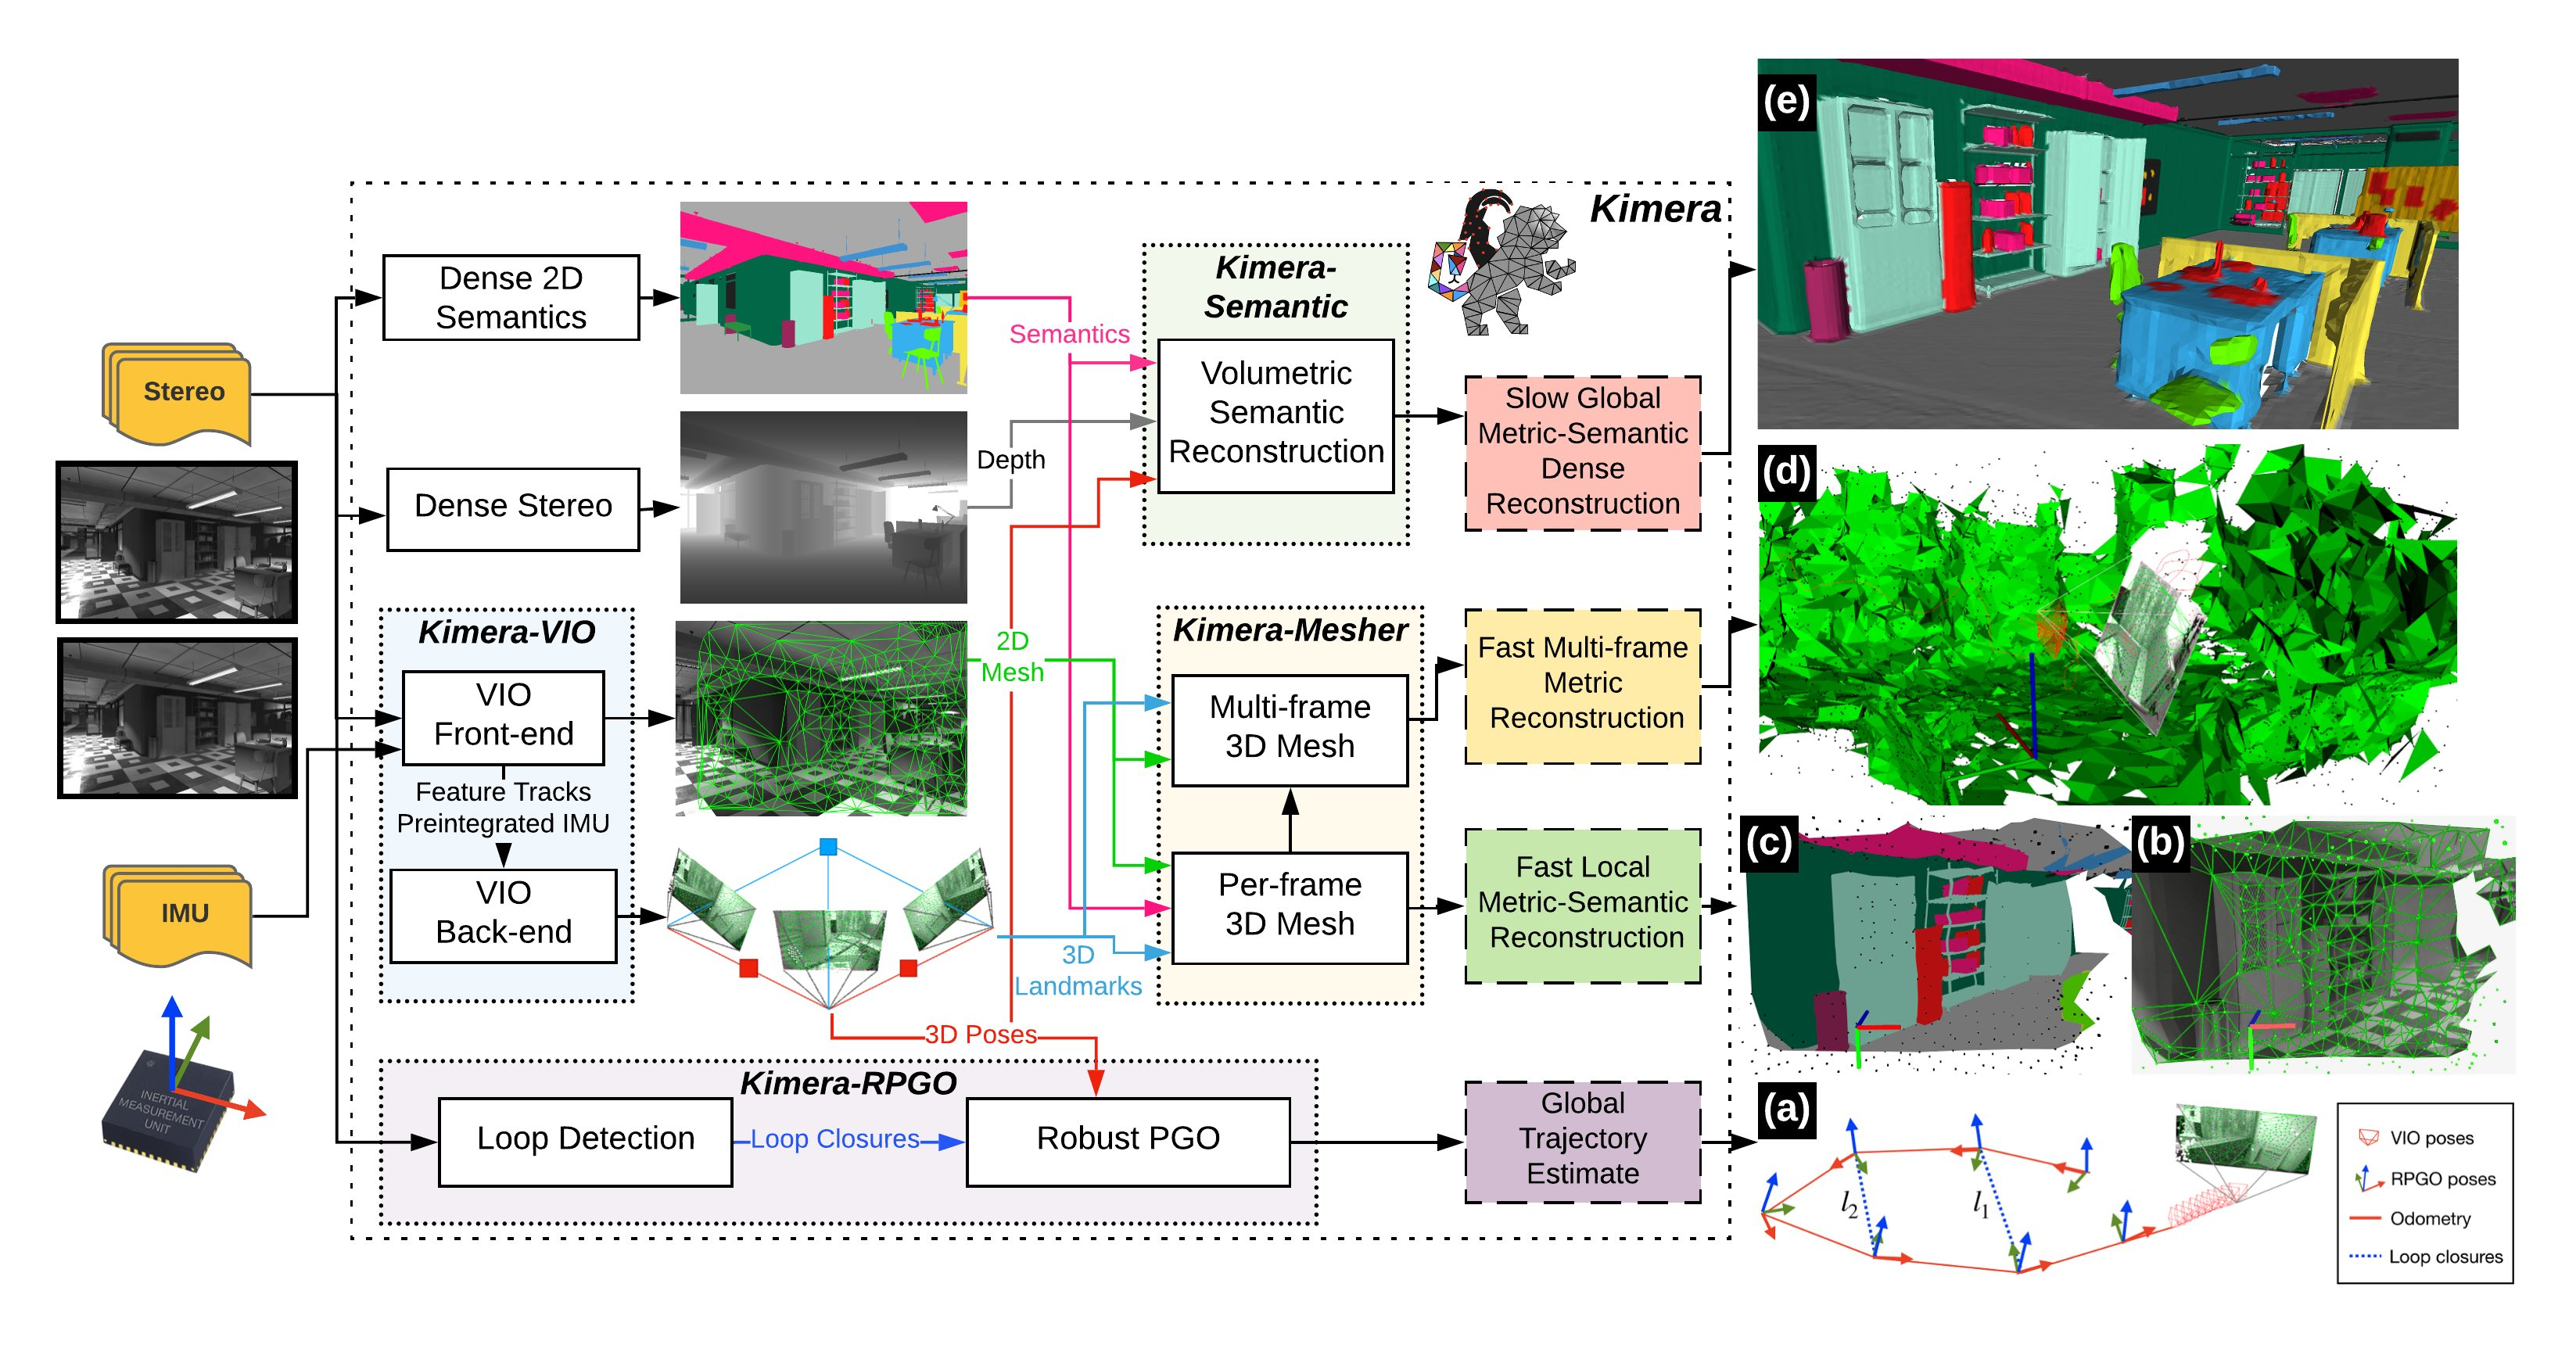
\includegraphics[width=\linewidth]{kimera_chart_23.jpeg} 
\end{figure}
\end{frame}
\begin{frame}
\frametitle{Kimera-Mesher}
\begin{figure}
    \includegraphics[width=\linewidth]{kimera_chart_Mesher.jpeg} 
\end{figure}
\end{frame}
\begin{frame}
\frametitle{Kimera-Mesher}
\begin{minipage}{0.49\textwidth}
    \begin{figure}
        \includegraphics[width=\textwidth]{480px-Delaunay_circumcircles_vectorial.svg.png} 
        \caption{Delaunay Triangulation}
    \end{figure}
\end{minipage}
\begin{minipage}{0.49\textwidth}
    \begin{figure}[ht]
        \centering
        \animategraphics[width=\textwidth,autoplay,loop]{5}{kiemra_mesher_gif/kimeravio_release-}{0}{258}
        \caption{An example of mesh generation}
    \end{figure}
\end{minipage}
\end{frame}
\begin{frame}
\frametitle{The structure of Kimera}
\begin{figure}
    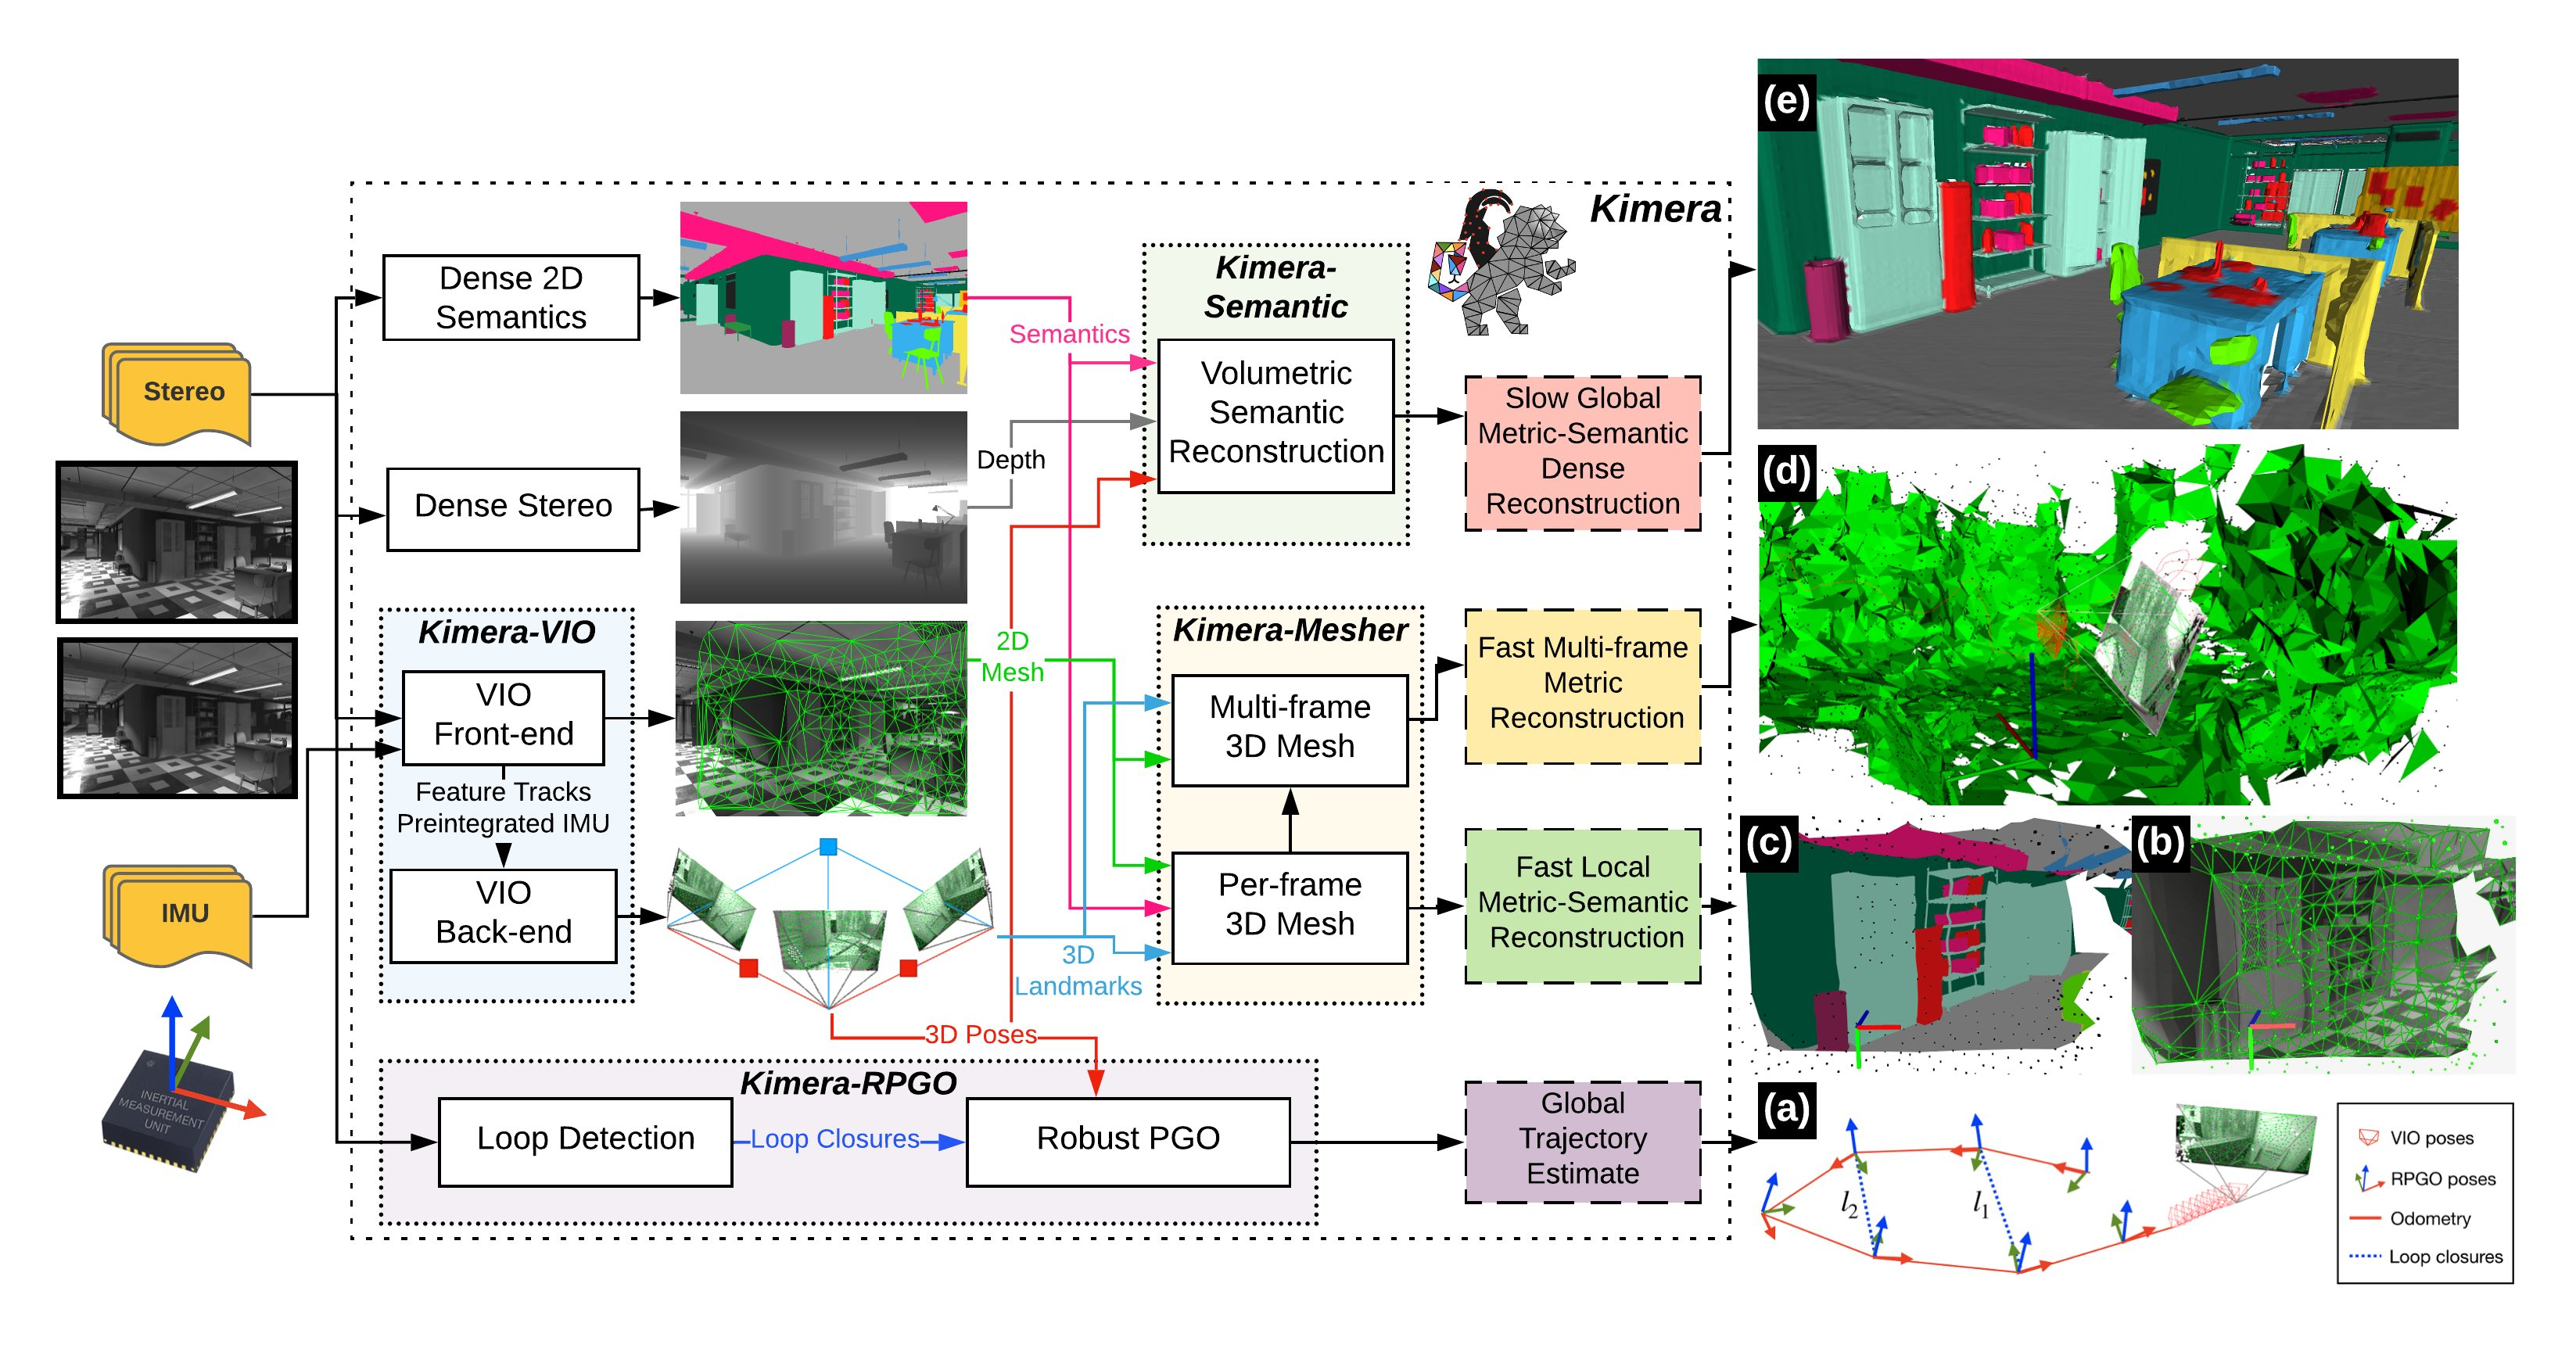
\includegraphics[width=\linewidth]{kimera_chart_23.jpeg} 
\end{figure}
\end{frame}
\begin{frame}
\frametitle{Kimera-Semantics}
\begin{figure}
    \includegraphics[width=\linewidth]{kimera_chart_Semantics.jpeg} 
\end{figure}
\end{frame}
\begin{frame}
\frametitle{Kimera-Semantics}
\begin{figure}
    \includegraphics[width=0.8\linewidth]{screenshot_2024-01-20-202326.png} 
    \caption{Semi global matching \cite{SGM}}
\end{figure}
\begin{figure}
    \includegraphics[width=0.5\linewidth]{MarchingCubesCases.png} 
    \caption{The 15 basic shapes of marching cubes \cite{marchingCubesImage} }
\end{figure}
\end{frame}
\begin{frame}
\frametitle{Kimera-Semantics}
    \begin{figure}[ht]
        \centering
        \animategraphics[width=\textwidth,autoplay,loop]{20}{kimera_semantics_gif/kimera_semantics-}{0}{387}
    \end{figure}
\end{frame}
\begin{frame}
\frametitle{What does Kimera do?}
\begin{figure}
    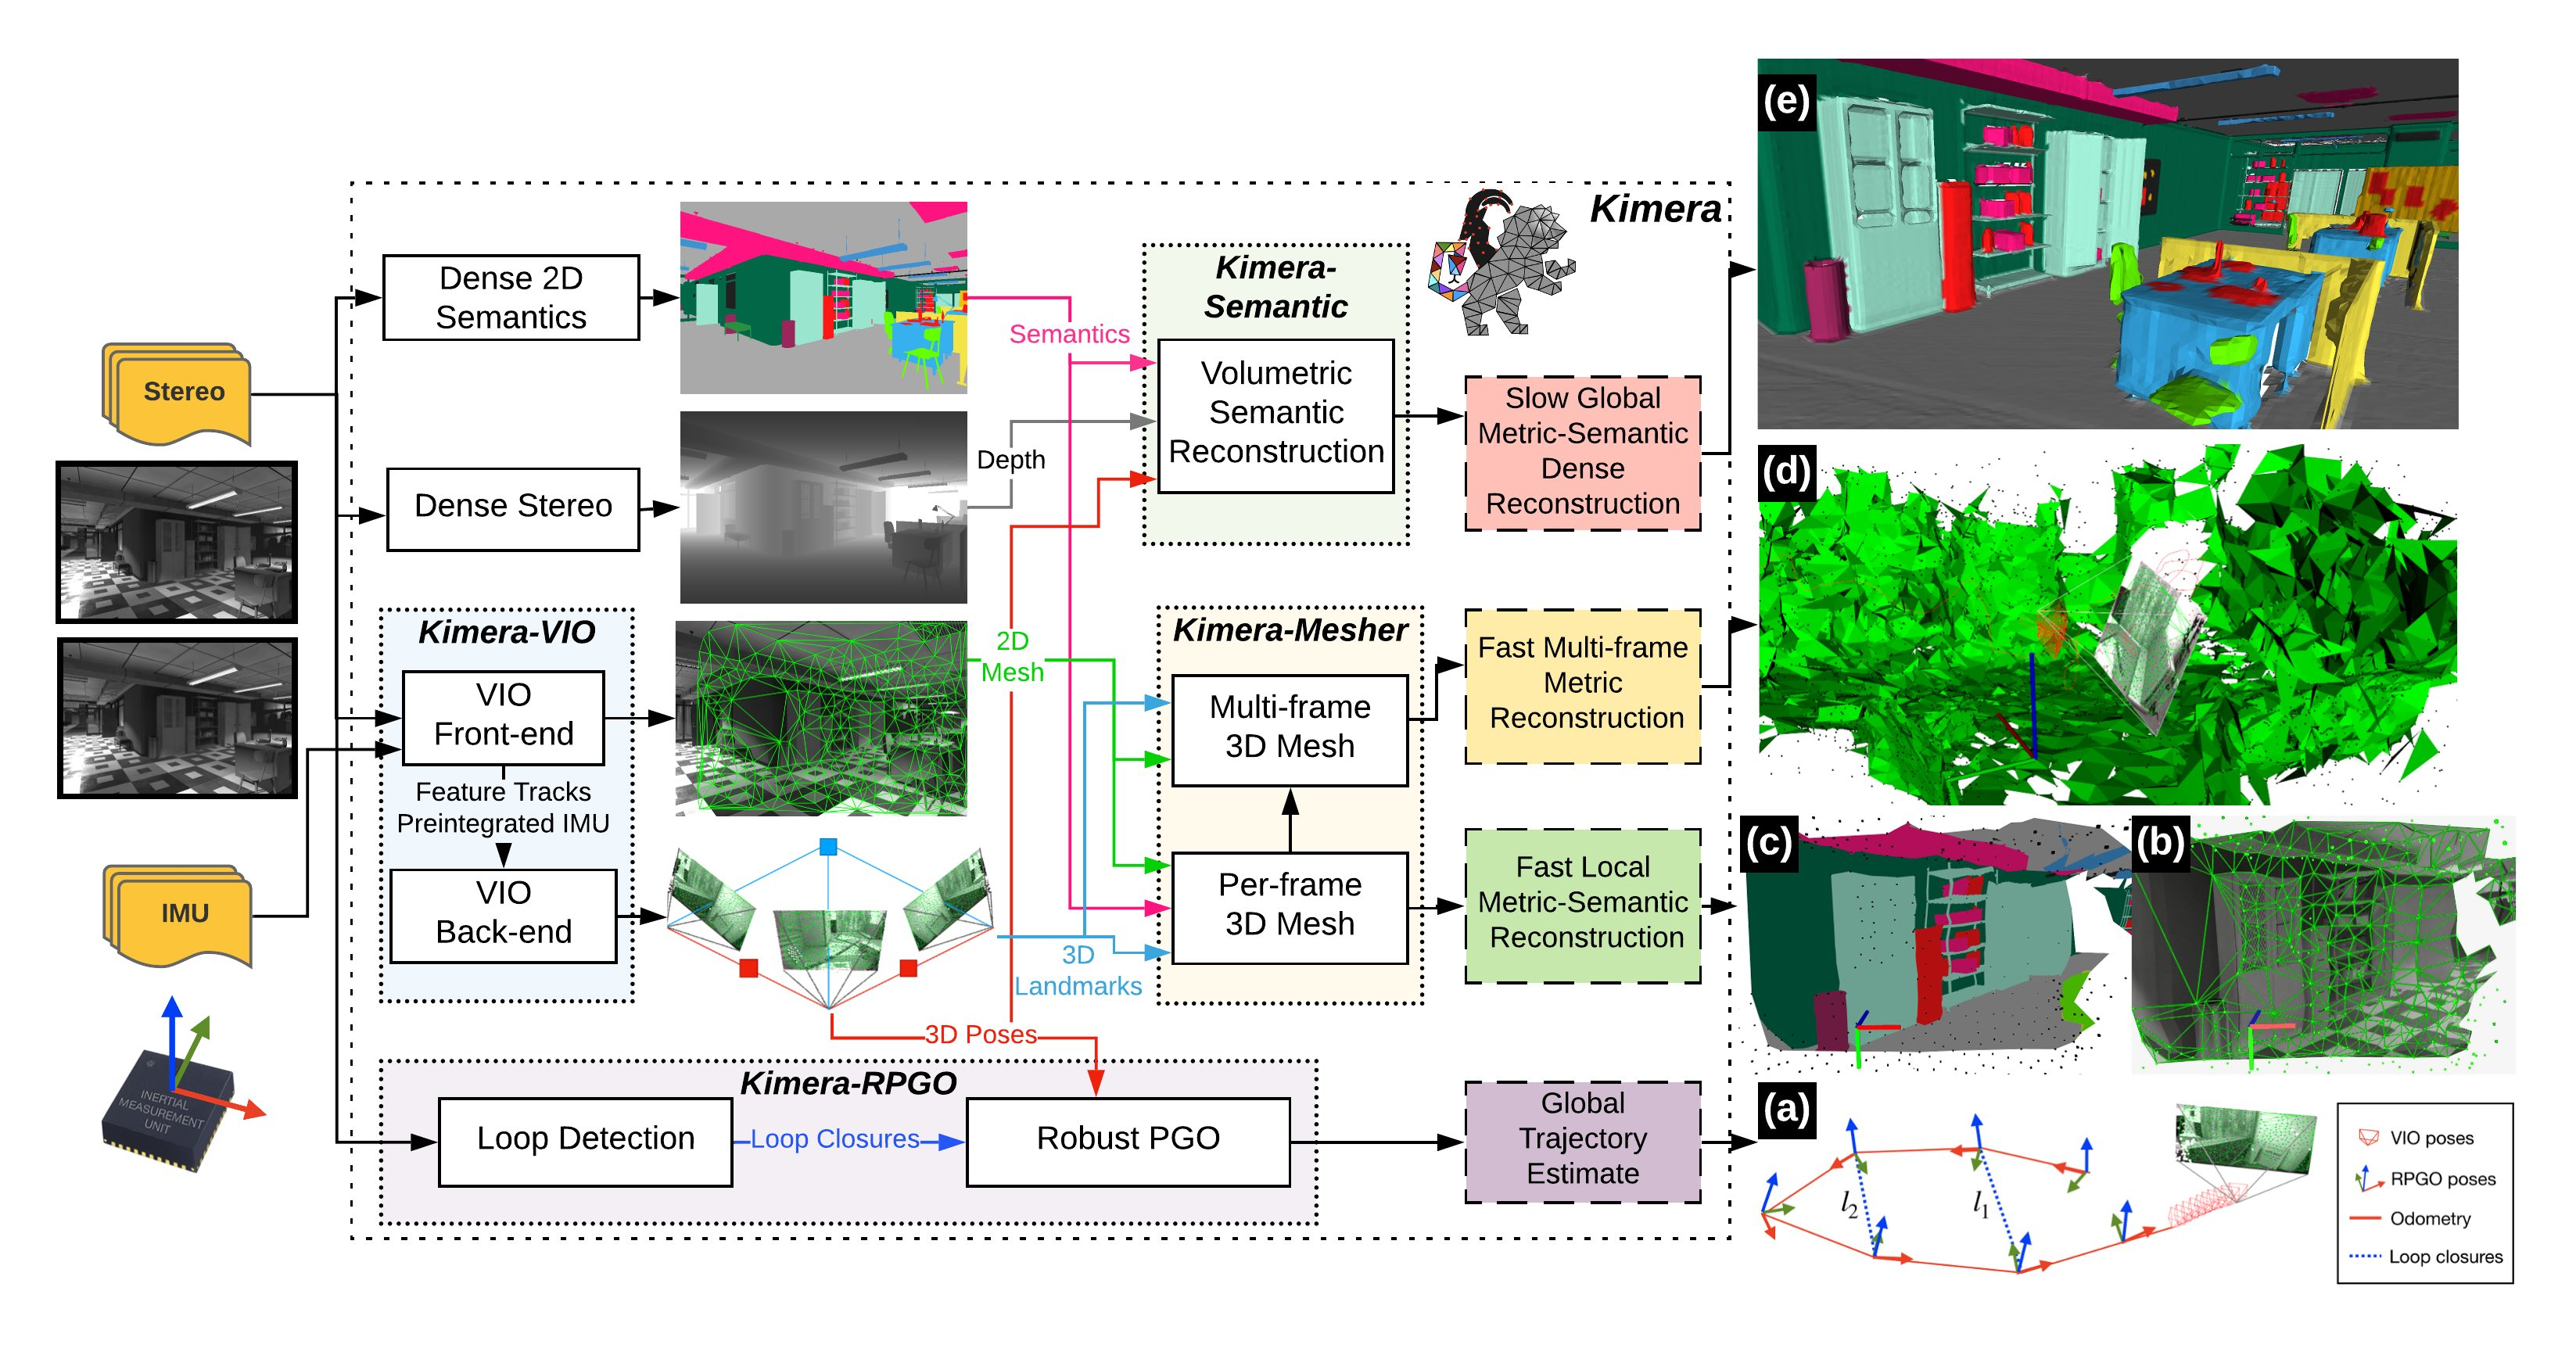
\includegraphics[width=\linewidth]{kimera_chart_23.jpeg} 
\end{figure}
\end{frame}
\begin{frame}
\frametitle{Performance}
\begin{minipage}{0.49\textwidth}
\begin{figure}
    \includegraphics[width=\linewidth]{screenshot_2024-01-24-191126.png} 
    \caption{Performance of Pose estimation}
\end{figure}
\end{minipage}
\begin{minipage}{0.49\textwidth}
\begin{figure}
    \includegraphics[width=\linewidth]{screenshot_2024-01-24-211538.png} 
    \caption{Performance of mesh reconstruction}
\end{figure}
\begin{figure}
    \includegraphics[width=\linewidth]{screenshot_2024-01-24-211639.png} 
    \caption{Comparison of Point reconstruction to ground truth}
\end{figure}
\end{minipage}
\end{frame}
\begin{frame}[allowframebreaks]
\footnotesize
  \frametitle{References}
  \bibliographystyle{plain}
\bibliography{paper}{}
\end{frame}

\end{document}
